% Created by tikzDevice version 0.12.6 on 2024-10-07 12:10:30
% !TEX encoding = UTF-8 Unicode
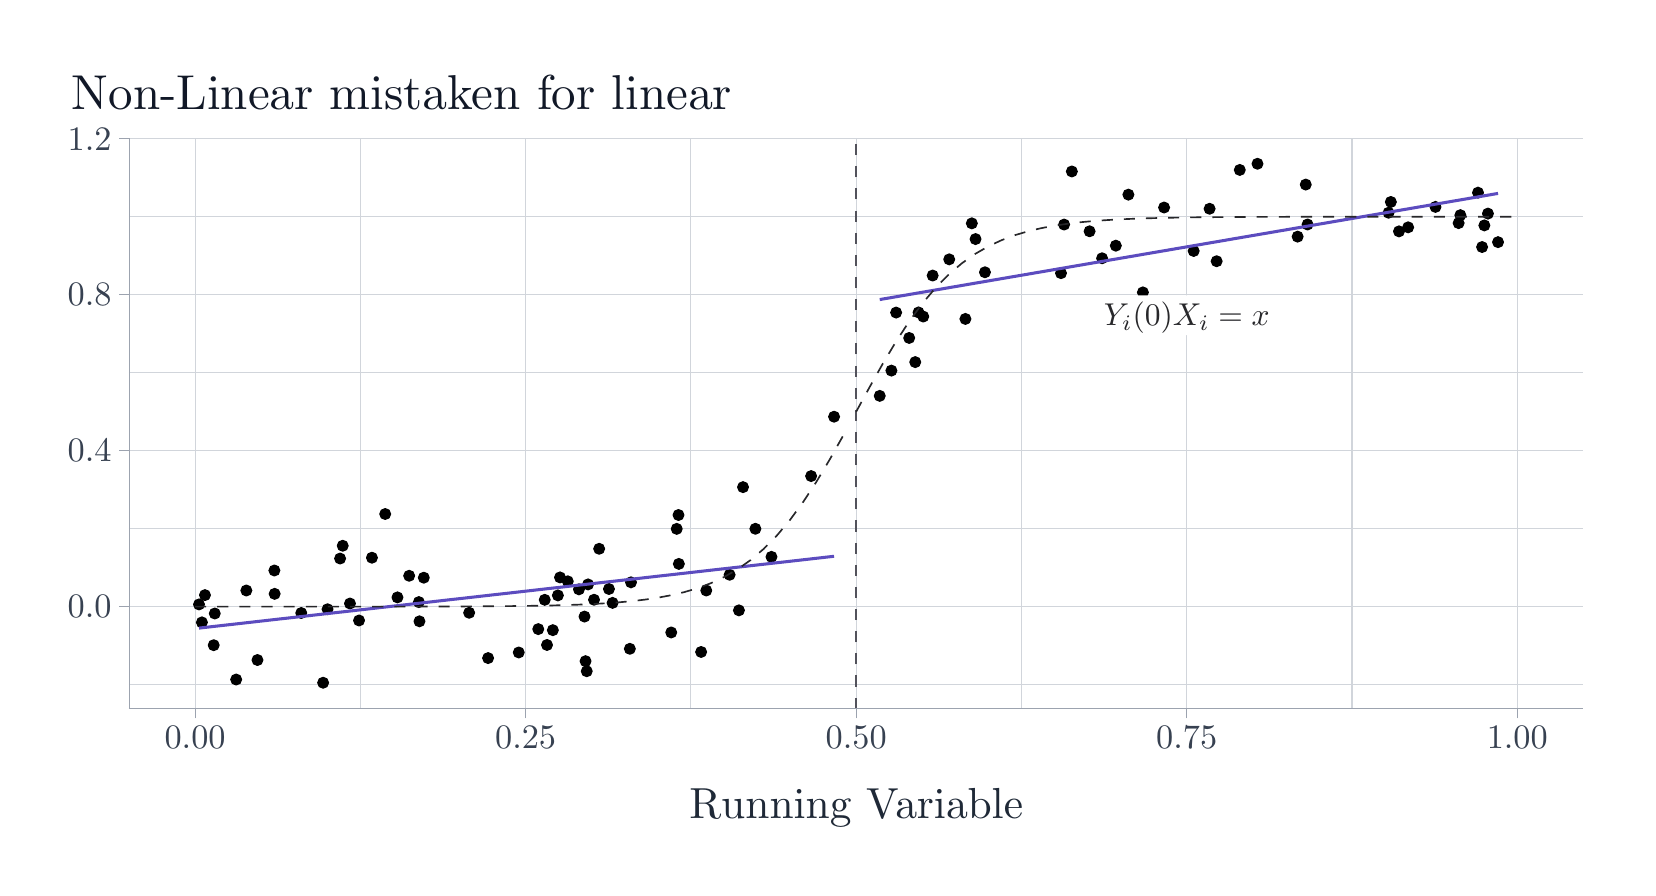
\begin{tikzpicture}[x=1pt,y=1pt]
\definecolor{fillColor}{RGB}{255,255,255}
\path[use as bounding box,fill=fillColor] (0,0) rectangle (578.16,303.53);
\begin{scope}
\path[clip] (  0.00,  0.00) rectangle (578.16,303.53);
\definecolor{drawColor}{RGB}{255,255,255}

\path[draw=drawColor,line width= 0.7pt,line join=round,line cap=round,fill=fillColor] (  0.00,  0.00) rectangle (578.16,303.53);
\end{scope}
\begin{scope}
\path[clip] ( 36.61, 57.45) rectangle (562.16,263.73);
\definecolor{drawColor}{RGB}{255,255,255}
\definecolor{fillColor}{RGB}{255,255,255}

\path[draw=drawColor,line width= 0.7pt,line join=round,line cap=round,fill=fillColor] ( 36.61, 57.45) rectangle (562.16,263.73);
\definecolor{drawColor}{RGB}{209,213,219}

\path[draw=drawColor,line width= 0.4pt,line join=round] ( 36.61, 66.13) --
	(562.16, 66.13);

\path[draw=drawColor,line width= 0.4pt,line join=round] ( 36.61,122.49) --
	(562.16,122.49);

\path[draw=drawColor,line width= 0.4pt,line join=round] ( 36.61,178.85) --
	(562.16,178.85);

\path[draw=drawColor,line width= 0.4pt,line join=round] ( 36.61,235.22) --
	(562.16,235.22);

\path[draw=drawColor,line width= 0.4pt,line join=round] (120.22, 57.45) --
	(120.22,263.73);

\path[draw=drawColor,line width= 0.4pt,line join=round] (239.66, 57.45) --
	(239.66,263.73);

\path[draw=drawColor,line width= 0.4pt,line join=round] (359.11, 57.45) --
	(359.11,263.73);

\path[draw=drawColor,line width= 0.4pt,line join=round] (478.55, 57.45) --
	(478.55,263.73);

\path[draw=drawColor,line width= 0.4pt,line join=round] ( 36.61, 94.31) --
	(562.16, 94.31);

\path[draw=drawColor,line width= 0.4pt,line join=round] ( 36.61,150.67) --
	(562.16,150.67);

\path[draw=drawColor,line width= 0.4pt,line join=round] ( 36.61,207.04) --
	(562.16,207.04);

\path[draw=drawColor,line width= 0.4pt,line join=round] ( 36.61,263.40) --
	(562.16,263.40);

\path[draw=drawColor,line width= 0.4pt,line join=round] ( 60.49, 57.45) --
	( 60.49,263.73);

\path[draw=drawColor,line width= 0.4pt,line join=round] (179.94, 57.45) --
	(179.94,263.73);

\path[draw=drawColor,line width= 0.4pt,line join=round] (299.38, 57.45) --
	(299.38,263.73);

\path[draw=drawColor,line width= 0.4pt,line join=round] (418.83, 57.45) --
	(418.83,263.73);

\path[draw=drawColor,line width= 0.4pt,line join=round] (538.27, 57.45) --
	(538.27,263.73);
\definecolor{drawColor}{RGB}{82,82,91}

\path[draw=drawColor,line width= 0.6pt,dash pattern=on 4pt off 4pt ,line join=round] (299.38, 57.45) -- (299.38,263.73);
\definecolor{drawColor}{RGB}{0,0,0}
\definecolor{fillColor}{RGB}{0,0,0}

\path[draw=drawColor,line width= 0.4pt,line join=round,line cap=round,fill=fillColor] ( 75.34, 67.98) circle (  1.96);

\path[draw=drawColor,line width= 0.4pt,line join=round,line cap=round,fill=fillColor] (206.51,115.22) circle (  1.96);

\path[draw=drawColor,line width= 0.4pt,line join=round,line cap=round,fill=fillColor] (201.59, 74.62) circle (  1.96);

\path[draw=drawColor,line width= 0.4pt,line join=round,line cap=round,fill=fillColor] ( 83.03, 75.03) circle (  1.96);

\path[draw=drawColor,line width= 0.4pt,line join=round,line cap=round,fill=fillColor] (257.01, 92.98) circle (  1.96);

\path[draw=drawColor,line width= 0.4pt,line join=round,line cap=round,fill=fillColor] (204.65, 96.81) circle (  1.96);

\path[draw=drawColor,line width= 0.4pt,line join=round,line cap=round,fill=fillColor] ( 98.86, 92.02) circle (  1.96);

\path[draw=drawColor,line width= 0.4pt,line join=round,line cap=round,fill=fillColor] ( 64.06, 98.49) circle (  1.96);

\path[draw=drawColor,line width= 0.4pt,line join=round,line cap=round,fill=fillColor] (191.59, 98.38) circle (  1.96);

\path[draw=drawColor,line width= 0.4pt,line join=round,line cap=round,fill=fillColor] (195.16,103.47) circle (  1.96);

\path[draw=drawColor,line width= 0.4pt,line join=round,line cap=round,fill=fillColor] (527.66,236.34) circle (  1.96);

\path[draw=drawColor,line width= 0.4pt,line join=round,line cap=round,fill=fillColor] (232.55, 84.99) circle (  1.96);

\path[draw=drawColor,line width= 0.4pt,line join=round,line cap=round,fill=fillColor] (508.71,238.76) circle (  1.96);

\path[draw=drawColor,line width= 0.4pt,line join=round,line cap=round,fill=fillColor] (211.35, 95.68) circle (  1.96);

\path[draw=drawColor,line width= 0.4pt,line join=round,line cap=round,fill=fillColor] (234.53,122.42) circle (  1.96);

\path[draw=drawColor,line width= 0.4pt,line join=round,line cap=round,fill=fillColor] (374.51,232.38) circle (  1.96);

\path[draw=drawColor,line width= 0.4pt,line join=round,line cap=round,fill=fillColor] ( 89.15,107.38) circle (  1.96);

\path[draw=drawColor,line width= 0.4pt,line join=round,line cap=round,fill=fillColor] (402.98,207.87) circle (  1.96);

\path[draw=drawColor,line width= 0.4pt,line join=round,line cap=round,fill=fillColor] (177.45, 77.76) circle (  1.96);

\path[draw=drawColor,line width= 0.4pt,line join=round,line cap=round,fill=fillColor] (393.20,224.75) circle (  1.96);

\path[draw=drawColor,line width= 0.4pt,line join=round,line cap=round,fill=fillColor] (323.62,199.14) circle (  1.96);

\path[draw=drawColor,line width= 0.4pt,line join=round,line cap=round,fill=fillColor] (184.50, 86.20) circle (  1.96);

\path[draw=drawColor,line width= 0.4pt,line join=round,line cap=round,fill=fillColor] (253.64,105.83) circle (  1.96);

\path[draw=drawColor,line width= 0.4pt,line join=round,line cap=round,fill=fillColor] (262.96,122.45) circle (  1.96);

\path[draw=drawColor,line width= 0.4pt,line join=round,line cap=round,fill=fillColor] (318.53,191.41) circle (  1.96);

\path[draw=drawColor,line width= 0.4pt,line join=round,line cap=round,fill=fillColor] ( 89.24, 98.94) circle (  1.96);

\path[draw=drawColor,line width= 0.4pt,line join=round,line cap=round,fill=fillColor] (524.07,243.91) circle (  1.96);

\path[draw=drawColor,line width= 0.4pt,line join=round,line cap=round,fill=fillColor] (462.48,232.41) circle (  1.96);

\path[draw=drawColor,line width= 0.4pt,line join=round,line cap=round,fill=fillColor] (321.91,200.63) circle (  1.96);

\path[draw=drawColor,line width= 0.4pt,line join=round,line cap=round,fill=fillColor] (525.55,224.26) circle (  1.96);

\path[draw=drawColor,line width= 0.4pt,line join=round,line cap=round,fill=fillColor] (245.21,100.15) circle (  1.96);

\path[draw=drawColor,line width= 0.4pt,line join=round,line cap=round,fill=fillColor] (421.33,222.84) circle (  1.96);

\path[draw=drawColor,line width= 0.4pt,line join=round,line cap=round,fill=fillColor] (410.64,238.54) circle (  1.96);

\path[draw=drawColor,line width= 0.4pt,line join=round,line cap=round,fill=fillColor] (143.14,104.78) circle (  1.96);

\path[draw=drawColor,line width= 0.4pt,line join=round,line cap=round,fill=fillColor] ( 62.96, 88.63) circle (  1.96);

\path[draw=drawColor,line width= 0.4pt,line join=round,line cap=round,fill=fillColor] (312.11,179.61) circle (  1.96);

\path[draw=drawColor,line width= 0.4pt,line join=round,line cap=round,fill=fillColor] ( 67.22, 80.39) circle (  1.96);

\path[draw=drawColor,line width= 0.4pt,line join=round,line cap=round,fill=fillColor] (235.30,109.76) circle (  1.96);

\path[draw=drawColor,line width= 0.4pt,line join=round,line cap=round,fill=fillColor] (113.84,116.32) circle (  1.96);

\path[draw=drawColor,line width= 0.4pt,line join=round,line cap=round,fill=fillColor] (106.76, 66.82) circle (  1.96);

\path[draw=drawColor,line width= 0.4pt,line join=round,line cap=round,fill=fillColor] (192.36,104.88) circle (  1.96);

\path[draw=drawColor,line width= 0.4pt,line join=round,line cap=round,fill=fillColor] (119.74, 89.32) circle (  1.96);

\path[draw=drawColor,line width= 0.4pt,line join=round,line cap=round,fill=fillColor] ( 79.02,100.15) circle (  1.96);

\path[draw=drawColor,line width= 0.4pt,line join=round,line cap=round,fill=fillColor] (345.91,215.14) circle (  1.96);

\path[draw=drawColor,line width= 0.4pt,line join=round,line cap=round,fill=fillColor] (166.37, 75.73) circle (  1.96);

\path[draw=drawColor,line width= 0.4pt,line join=round,line cap=round,fill=fillColor] (342.51,227.14) circle (  1.96);

\path[draw=drawColor,line width= 0.4pt,line join=round,line cap=round,fill=fillColor] (202.49,102.35) circle (  1.96);

\path[draw=drawColor,line width= 0.4pt,line join=round,line cap=round,fill=fillColor] (129.19,127.79) circle (  1.96);

\path[draw=drawColor,line width= 0.4pt,line join=round,line cap=round,fill=fillColor] (427.08,238.09) circle (  1.96);

\path[draw=drawColor,line width= 0.4pt,line join=round,line cap=round,fill=fillColor] (133.62, 97.66) circle (  1.96);

\path[draw=drawColor,line width= 0.4pt,line join=round,line cap=round,fill=fillColor] (137.85,105.47) circle (  1.96);

\path[draw=drawColor,line width= 0.4pt,line join=round,line cap=round,fill=fillColor] (112.89,111.70) circle (  1.96);

\path[draw=drawColor,line width= 0.4pt,line join=round,line cap=round,fill=fillColor] (218.01,103.10) circle (  1.96);

\path[draw=drawColor,line width= 0.4pt,line join=round,line cap=round,fill=fillColor] (498.83,231.38) circle (  1.96);

\path[draw=drawColor,line width= 0.4pt,line join=round,line cap=round,fill=fillColor] (388.24,220.20) circle (  1.96);

\path[draw=drawColor,line width= 0.4pt,line join=round,line cap=round,fill=fillColor] (210.04,100.69) circle (  1.96);

\path[draw=drawColor,line width= 0.4pt,line join=round,line cap=round,fill=fillColor] (461.83,246.83) circle (  1.96);

\path[draw=drawColor,line width= 0.4pt,line join=round,line cap=round,fill=fillColor] (201.21, 90.73) circle (  1.96);

\path[draw=drawColor,line width= 0.4pt,line join=round,line cap=round,fill=fillColor] (429.63,219.13) circle (  1.96);

\path[draw=drawColor,line width= 0.4pt,line join=round,line cap=round,fill=fillColor] (313.81,200.58) circle (  1.96);

\path[draw=drawColor,line width= 0.4pt,line join=round,line cap=round,fill=fillColor] (491.75,236.65) circle (  1.96);

\path[draw=drawColor,line width= 0.4pt,line join=round,line cap=round,fill=fillColor] (258.49,137.50) circle (  1.96);

\path[draw=drawColor,line width= 0.4pt,line join=round,line cap=round,fill=fillColor] (108.36, 93.38) circle (  1.96);

\path[draw=drawColor,line width= 0.4pt,line join=round,line cap=round,fill=fillColor] (327.01,213.96) circle (  1.96);

\path[draw=drawColor,line width= 0.4pt,line join=round,line cap=round,fill=fillColor] (235.17,127.43) circle (  1.96);

\path[draw=drawColor,line width= 0.4pt,line join=round,line cap=round,fill=fillColor] (243.35, 77.94) circle (  1.96);

\path[draw=drawColor,line width= 0.4pt,line join=round,line cap=round,fill=fillColor] (141.36, 95.97) circle (  1.96);

\path[draw=drawColor,line width= 0.4pt,line join=round,line cap=round,fill=fillColor] (341.17,232.82) circle (  1.96);

\path[draw=drawColor,line width= 0.4pt,line join=round,line cap=round,fill=fillColor] (202.02, 70.98) circle (  1.96);

\path[draw=drawColor,line width= 0.4pt,line join=round,line cap=round,fill=fillColor] (383.72,229.95) circle (  1.96);

\path[draw=drawColor,line width= 0.4pt,line join=round,line cap=round,fill=fillColor] (124.40,112.00) circle (  1.96);

\path[draw=drawColor,line width= 0.4pt,line join=round,line cap=round,fill=fillColor] (189.77, 85.82) circle (  1.96);

\path[draw=drawColor,line width= 0.4pt,line join=round,line cap=round,fill=fillColor] (268.77,112.31) circle (  1.96);

\path[draw=drawColor,line width= 0.4pt,line join=round,line cap=round,fill=fillColor] (458.89,228.02) circle (  1.96);

\path[draw=drawColor,line width= 0.4pt,line join=round,line cap=round,fill=fillColor] (531.31,226.03) circle (  1.96);

\path[draw=drawColor,line width= 0.4pt,line join=round,line cap=round,fill=fillColor] (141.57, 89.01) circle (  1.96);

\path[draw=drawColor,line width= 0.4pt,line join=round,line cap=round,fill=fillColor] (526.37,232.08) circle (  1.96);

\path[draw=drawColor,line width= 0.4pt,line join=round,line cap=round,fill=fillColor] (444.39,254.35) circle (  1.96);

\path[draw=drawColor,line width= 0.4pt,line join=round,line cap=round,fill=fillColor] (116.46, 95.45) circle (  1.96);

\path[draw=drawColor,line width= 0.4pt,line join=round,line cap=round,fill=fillColor] (320.72,182.68) circle (  1.96);

\path[draw=drawColor,line width= 0.4pt,line join=round,line cap=round,fill=fillColor] (186.84, 96.78) circle (  1.96);

\path[draw=drawColor,line width= 0.4pt,line join=round,line cap=round,fill=fillColor] (492.58,240.55) circle (  1.96);

\path[draw=drawColor,line width= 0.4pt,line join=round,line cap=round,fill=fillColor] (199.20,100.57) circle (  1.96);

\path[draw=drawColor,line width= 0.4pt,line join=round,line cap=round,fill=fillColor] (187.66, 80.47) circle (  1.96);

\path[draw=drawColor,line width= 0.4pt,line join=round,line cap=round,fill=fillColor] (283.10,141.50) circle (  1.96);

\path[draw=drawColor,line width= 0.4pt,line join=round,line cap=round,fill=fillColor] (159.53, 92.10) circle (  1.96);

\path[draw=drawColor,line width= 0.4pt,line join=round,line cap=round,fill=fillColor] (333.00,219.81) circle (  1.96);

\path[draw=drawColor,line width= 0.4pt,line join=round,line cap=round,fill=fillColor] (517.07,232.91) circle (  1.96);

\path[draw=drawColor,line width= 0.4pt,line join=round,line cap=round,fill=fillColor] ( 61.91, 95.12) circle (  1.96);

\path[draw=drawColor,line width= 0.4pt,line join=round,line cap=round,fill=fillColor] (517.70,235.78) circle (  1.96);

\path[draw=drawColor,line width= 0.4pt,line join=round,line cap=round,fill=fillColor] (377.31,251.57) circle (  1.96);

\path[draw=drawColor,line width= 0.4pt,line join=round,line cap=round,fill=fillColor] (495.52,229.92) circle (  1.96);

\path[draw=drawColor,line width= 0.4pt,line join=round,line cap=round,fill=fillColor] (373.39,214.82) circle (  1.96);

\path[draw=drawColor,line width= 0.4pt,line join=round,line cap=round,fill=fillColor] ( 67.61, 91.84) circle (  1.96);

\path[draw=drawColor,line width= 0.4pt,line join=round,line cap=round,fill=fillColor] (397.74,243.19) circle (  1.96);

\path[draw=drawColor,line width= 0.4pt,line join=round,line cap=round,fill=fillColor] (291.39,162.95) circle (  1.96);

\path[draw=drawColor,line width= 0.4pt,line join=round,line cap=round,fill=fillColor] (217.59, 79.08) circle (  1.96);

\path[draw=drawColor,line width= 0.4pt,line join=round,line cap=round,fill=fillColor] (437.99,252.12) circle (  1.96);

\path[draw=drawColor,line width= 0.4pt,line join=round,line cap=round,fill=fillColor] (338.85,198.28) circle (  1.96);

\path[draw=drawColor,line width= 0.4pt,line join=round,line cap=round,fill=fillColor] (307.89,170.48) circle (  1.96);
\definecolor{drawColor}{RGB}{92,76,191}

\path[draw=drawColor,line width= 1.1pt,line join=round] ( 61.91, 86.56) --
	( 64.81, 86.89) --
	( 67.72, 87.22) --
	( 70.62, 87.55) --
	( 73.53, 87.87) --
	( 76.43, 88.20) --
	( 79.34, 88.53) --
	( 82.24, 88.86) --
	( 85.15, 89.19) --
	( 88.05, 89.52) --
	( 90.96, 89.85) --
	( 93.86, 90.17) --
	( 96.77, 90.50) --
	( 99.67, 90.83) --
	(102.57, 91.16) --
	(105.48, 91.49) --
	(108.38, 91.82) --
	(111.29, 92.15) --
	(114.19, 92.47) --
	(117.10, 92.80) --
	(120.00, 93.13) --
	(122.91, 93.46) --
	(125.81, 93.79) --
	(128.72, 94.12) --
	(131.62, 94.45) --
	(134.53, 94.77) --
	(137.43, 95.10) --
	(140.34, 95.43) --
	(143.24, 95.76) --
	(146.15, 96.09) --
	(149.05, 96.42) --
	(151.96, 96.75) --
	(154.86, 97.07) --
	(157.77, 97.40) --
	(160.67, 97.73) --
	(163.58, 98.06) --
	(166.48, 98.39) --
	(169.39, 98.72) --
	(172.29, 99.04) --
	(175.20, 99.37) --
	(178.10, 99.70) --
	(181.01,100.03) --
	(183.91,100.36) --
	(186.82,100.69) --
	(189.72,101.02) --
	(192.63,101.34) --
	(195.53,101.67) --
	(198.44,102.00) --
	(201.34,102.33) --
	(204.24,102.66) --
	(207.15,102.99) --
	(210.05,103.32) --
	(212.96,103.64) --
	(215.86,103.97) --
	(218.77,104.30) --
	(221.67,104.63) --
	(224.58,104.96) --
	(227.48,105.29) --
	(230.39,105.62) --
	(233.29,105.94) --
	(236.20,106.27) --
	(239.10,106.60) --
	(242.01,106.93) --
	(244.91,107.26) --
	(247.82,107.59) --
	(250.72,107.92) --
	(253.63,108.24) --
	(256.53,108.57) --
	(259.44,108.90) --
	(262.34,109.23) --
	(265.25,109.56) --
	(268.15,109.89) --
	(271.06,110.22) --
	(273.96,110.54) --
	(276.87,110.87) --
	(279.77,111.20) --
	(282.68,111.53) --
	(285.58,111.86) --
	(288.49,112.19) --
	(291.39,112.52);

\path[draw=drawColor,line width= 1.1pt,line join=round] (307.89,205.28) --
	(310.72,205.77) --
	(313.55,206.25) --
	(316.38,206.74) --
	(319.20,207.22) --
	(322.03,207.71) --
	(324.86,208.19) --
	(327.69,208.68) --
	(330.52,209.16) --
	(333.34,209.65) --
	(336.17,210.13) --
	(339.00,210.62) --
	(341.83,211.11) --
	(344.66,211.59) --
	(347.48,212.08) --
	(350.31,212.56) --
	(353.14,213.05) --
	(355.97,213.53) --
	(358.80,214.02) --
	(361.63,214.50) --
	(364.45,214.99) --
	(367.28,215.47) --
	(370.11,215.96) --
	(372.94,216.45) --
	(375.77,216.93) --
	(378.59,217.42) --
	(381.42,217.90) --
	(384.25,218.39) --
	(387.08,218.87) --
	(389.91,219.36) --
	(392.73,219.84) --
	(395.56,220.33) --
	(398.39,220.81) --
	(401.22,221.30) --
	(404.05,221.79) --
	(406.88,222.27) --
	(409.70,222.76) --
	(412.53,223.24) --
	(415.36,223.73) --
	(418.19,224.21) --
	(421.02,224.70) --
	(423.84,225.18) --
	(426.67,225.67) --
	(429.50,226.15) --
	(432.33,226.64) --
	(435.16,227.13) --
	(437.98,227.61) --
	(440.81,228.10) --
	(443.64,228.58) --
	(446.47,229.07) --
	(449.30,229.55) --
	(452.13,230.04) --
	(454.95,230.52) --
	(457.78,231.01) --
	(460.61,231.49) --
	(463.44,231.98) --
	(466.27,232.47) --
	(469.09,232.95) --
	(471.92,233.44) --
	(474.75,233.92) --
	(477.58,234.41) --
	(480.41,234.89) --
	(483.23,235.38) --
	(486.06,235.86) --
	(488.89,236.35) --
	(491.72,236.83) --
	(494.55,237.32) --
	(497.38,237.81) --
	(500.20,238.29) --
	(503.03,238.78) --
	(505.86,239.26) --
	(508.69,239.75) --
	(511.52,240.23) --
	(514.34,240.72) --
	(517.17,241.20) --
	(520.00,241.69) --
	(522.83,242.17) --
	(525.66,242.66) --
	(528.48,243.15) --
	(531.31,243.63);
\definecolor{drawColor}{RGB}{39,39,42}

\path[draw=drawColor,line width= 0.6pt,dash pattern=on 4pt off 4pt ,line join=round] ( 60.49, 94.31) --
	( 65.27, 94.31) --
	( 70.05, 94.31) --
	( 74.83, 94.31) --
	( 79.61, 94.31) --
	( 84.38, 94.31) --
	( 89.16, 94.31) --
	( 93.94, 94.31) --
	( 98.72, 94.31) --
	(103.49, 94.31) --
	(108.27, 94.31) --
	(113.05, 94.32) --
	(117.83, 94.32) --
	(122.61, 94.32) --
	(127.38, 94.33) --
	(132.16, 94.33) --
	(136.94, 94.34) --
	(141.72, 94.34) --
	(146.49, 94.36) --
	(151.27, 94.37) --
	(156.05, 94.39) --
	(160.83, 94.41) --
	(165.61, 94.44) --
	(170.38, 94.47) --
	(175.16, 94.52) --
	(179.94, 94.58) --
	(184.72, 94.66) --
	(189.49, 94.75) --
	(194.27, 94.88) --
	(199.05, 95.04) --
	(203.83, 95.25) --
	(208.61, 95.52) --
	(213.38, 95.86) --
	(218.16, 96.29) --
	(222.94, 96.84) --
	(227.72, 97.55) --
	(232.49, 98.44) --
	(237.27, 99.57) --
	(242.05,100.99) --
	(246.83,102.77) --
	(251.61,105.00) --
	(256.38,107.74) --
	(261.16,111.10) --
	(265.94,115.17) --
	(270.72,120.01) --
	(275.49,125.69) --
	(280.27,132.20) --
	(285.05,139.51) --
	(289.83,147.51) --
	(294.61,156.00);

\path[draw=drawColor,line width= 0.6pt,dash pattern=on 4pt off 4pt ,line join=round] (299.38,164.76) --
	(304.16,173.52) --
	(308.94,182.02) --
	(313.72,190.01) --
	(318.49,197.32) --
	(323.27,203.84) --
	(328.05,209.51) --
	(332.83,214.36) --
	(337.61,218.42) --
	(342.38,221.78) --
	(347.16,224.53) --
	(351.94,226.75) --
	(356.72,228.54) --
	(361.49,229.96) --
	(366.27,231.09) --
	(371.05,231.98) --
	(375.83,232.68) --
	(380.60,233.24) --
	(385.38,233.67) --
	(390.16,234.01) --
	(394.94,234.28) --
	(399.72,234.48) --
	(404.49,234.64) --
	(409.27,234.77) --
	(414.05,234.87) --
	(418.83,234.95) --
	(423.60,235.01) --
	(428.38,235.05) --
	(433.16,235.09) --
	(437.94,235.12) --
	(442.72,235.14) --
	(447.49,235.16) --
	(452.27,235.17) --
	(457.05,235.18) --
	(461.83,235.19) --
	(466.60,235.20) --
	(471.38,235.20) --
	(476.16,235.20) --
	(480.94,235.21) --
	(485.72,235.21) --
	(490.49,235.21) --
	(495.27,235.21) --
	(500.05,235.21) --
	(504.83,235.22) --
	(509.60,235.22) --
	(514.38,235.22) --
	(519.16,235.22) --
	(523.94,235.22) --
	(528.72,235.22) --
	(533.49,235.22) --
	(538.27,235.22);
\definecolor{fillColor}{RGB}{255,255,255}

\path[fill=fillColor] (375.21,192.45) --
	(462.44,192.45) --
	(462.36,192.45) --
	(462.69,192.46) --
	(463.01,192.53) --
	(463.32,192.64) --
	(463.61,192.81) --
	(463.87,193.02) --
	(464.09,193.27) --
	(464.26,193.55) --
	(464.39,193.85) --
	(464.47,194.17) --
	(464.50,194.50) --
	(464.50,194.50) --
	(464.50,204.71) --
	(464.50,204.71) --
	(464.47,205.04) --
	(464.39,205.36) --
	(464.26,205.66) --
	(464.09,205.94) --
	(463.87,206.19) --
	(463.61,206.40) --
	(463.32,206.57) --
	(463.01,206.68) --
	(462.69,206.75) --
	(462.44,206.76) --
	(375.21,206.76) --
	(375.46,206.75) --
	(375.13,206.76) --
	(374.80,206.72) --
	(374.48,206.63) --
	(374.18,206.49) --
	(373.91,206.30) --
	(373.67,206.07) --
	(373.47,205.81) --
	(373.32,205.51) --
	(373.22,205.20) --
	(373.16,204.87) --
	(373.16,204.71) --
	(373.16,194.50) --
	(373.16,194.67) --
	(373.16,194.34) --
	(373.22,194.01) --
	(373.32,193.70) --
	(373.47,193.40) --
	(373.67,193.14) --
	(373.91,192.91) --
	(374.18,192.72) --
	(374.48,192.58) --
	(374.80,192.49) --
	(375.13,192.45) --
	cycle;
\end{scope}
\begin{scope}
\path[clip] ( 36.61, 57.45) rectangle (562.16,263.73);
\definecolor{drawColor}{RGB}{0,0,0}

\node[text=drawColor,anchor=base,inner sep=0pt, outer sep=0pt, scale=  1.14] at (418.83,195.87) {\color[HTML]{27272a}{$\expec{ Y_i(0) }{ X_i = x }$}};
\end{scope}
\begin{scope}
\path[clip] (  0.00,  0.00) rectangle (578.16,303.53);
\definecolor{drawColor}{RGB}{156,163,175}

\path[draw=drawColor,line width= 0.3pt,line join=round] ( 36.61, 57.45) --
	( 36.61,263.73);
\end{scope}
\begin{scope}
\path[clip] (  0.00,  0.00) rectangle (578.16,303.53);
\definecolor{drawColor}{RGB}{55,65,81}

\node[text=drawColor,anchor=base east,inner sep=0pt, outer sep=0pt, scale=  1.24] at ( 30.31, 90.23) {0.0};

\node[text=drawColor,anchor=base east,inner sep=0pt, outer sep=0pt, scale=  1.24] at ( 30.31,146.59) {0.4};

\node[text=drawColor,anchor=base east,inner sep=0pt, outer sep=0pt, scale=  1.24] at ( 30.31,202.96) {0.8};

\node[text=drawColor,anchor=base east,inner sep=0pt, outer sep=0pt, scale=  1.24] at ( 30.31,259.32) {1.2};
\end{scope}
\begin{scope}
\path[clip] (  0.00,  0.00) rectangle (578.16,303.53);
\definecolor{drawColor}{RGB}{156,163,175}

\path[draw=drawColor,line width= 0.3pt,line join=round] ( 33.11, 94.31) --
	( 36.61, 94.31);

\path[draw=drawColor,line width= 0.3pt,line join=round] ( 33.11,150.67) --
	( 36.61,150.67);

\path[draw=drawColor,line width= 0.3pt,line join=round] ( 33.11,207.04) --
	( 36.61,207.04);

\path[draw=drawColor,line width= 0.3pt,line join=round] ( 33.11,263.40) --
	( 36.61,263.40);
\end{scope}
\begin{scope}
\path[clip] (  0.00,  0.00) rectangle (578.16,303.53);
\definecolor{drawColor}{RGB}{156,163,175}

\path[draw=drawColor,line width= 0.3pt,line join=round] ( 36.61, 57.45) --
	(562.16, 57.45);
\end{scope}
\begin{scope}
\path[clip] (  0.00,  0.00) rectangle (578.16,303.53);
\definecolor{drawColor}{RGB}{156,163,175}

\path[draw=drawColor,line width= 0.3pt,line join=round] ( 60.49, 53.95) --
	( 60.49, 57.45);

\path[draw=drawColor,line width= 0.3pt,line join=round] (179.94, 53.95) --
	(179.94, 57.45);

\path[draw=drawColor,line width= 0.3pt,line join=round] (299.38, 53.95) --
	(299.38, 57.45);

\path[draw=drawColor,line width= 0.3pt,line join=round] (418.83, 53.95) --
	(418.83, 57.45);

\path[draw=drawColor,line width= 0.3pt,line join=round] (538.27, 53.95) --
	(538.27, 57.45);
\end{scope}
\begin{scope}
\path[clip] (  0.00,  0.00) rectangle (578.16,303.53);
\definecolor{drawColor}{RGB}{55,65,81}

\node[text=drawColor,anchor=base,inner sep=0pt, outer sep=0pt, scale=  1.24] at ( 60.49, 42.98) {0.00};

\node[text=drawColor,anchor=base,inner sep=0pt, outer sep=0pt, scale=  1.24] at (179.94, 42.98) {0.25};

\node[text=drawColor,anchor=base,inner sep=0pt, outer sep=0pt, scale=  1.24] at (299.38, 42.98) {0.50};

\node[text=drawColor,anchor=base,inner sep=0pt, outer sep=0pt, scale=  1.24] at (418.83, 42.98) {0.75};

\node[text=drawColor,anchor=base,inner sep=0pt, outer sep=0pt, scale=  1.24] at (538.27, 42.98) {1.00};
\end{scope}
\begin{scope}
\path[clip] (  0.00,  0.00) rectangle (578.16,303.53);
\definecolor{drawColor}{RGB}{31,41,55}

\node[text=drawColor,anchor=base,inner sep=0pt, outer sep=0pt, scale=  1.57] at (299.38, 17.86) {Running Variable};
\end{scope}
\begin{scope}
\path[clip] (  0.00,  0.00) rectangle (578.16,303.53);
\definecolor{drawColor}{RGB}{17,24,39}

\node[text=drawColor,anchor=base west,inner sep=0pt, outer sep=0pt, scale=  1.77] at ( 16.00,273.82) {Non-Linear mistaken for linear};
\end{scope}
\end{tikzpicture}
